\documentclass[11pt, titlepage]{article}

\usepackage[margin=1in]{geometry}
\usepackage[strict]{changepage}
\usepackage{float}
\usepackage{fancyhdr}
\usepackage{mhchem}
\usepackage{siunitx}
\usepackage{wrapfig, booktabs}
\usepackage{enumitem}
\usepackage{caption}
\usepackage{commath}
\usepackage{amsmath}
\usepackage[hang]{footmisc}
\usepackage{multicol}
\usepackage{amsfonts}
\usepackage{mathrsfs}
\usepackage{mathtools}
\usepackage{tikz}

% my imports
\usepackage[most]{tcolorbox}
\usepackage{hyperref}
\hypersetup{
    colorlinks,
    citecolor=black,
    filecolor=black,
    linkcolor=black,
    urlcolor=black
}

\newcommand{\experimentDate}{\today}
\newcommand{\className}{CSE 371}
\newcommand{\assignmentname}{Lab 1}
\author{Cameron Jennings (ID: 2029631), Donovan Clay (ID: 2276005)}
\newcommand{\authorLastName}{Jennings, Clay}
\title{\assignmentname}

\date{\parbox{\linewidth}{\centering
\experimentDate
  \endgraf\bigskip
  \className\
}}

\pagestyle{fancy}
\fancyhf{}
\setlength{\headheight}{13.59999pt}
\rhead{\authorLastName\ \thepage}
% \lhead{\experimentShortName}
\lhead{\hyperref[beginning]{\assignmentname}}
\cfoot{\className\ -- \assignmentname}

\usepackage{color}
\usepackage{sectsty}

\definecolor{WordSectionBlue}{RGB}{30, 90, 147}

\allsectionsfont{\color{WordSectionBlue}}

\tcbuselibrary{breakable}


\begin{document}
	\maketitle
 
    \setcounter{tocdepth}{2}
    \begin{center}
        \tableofcontents\label{beginning}
    \end{center}
    \newpage
    
    \section{Design Procedure}
        In this lab we designed a parking lot system to keep track of the occupied spaces. There are two sensors, implemented with switches in a breadboard, one sensor is scanning the outside of the lot and one is scanning. The outside sensor connected to V\_GPIO[28] and the inner V\_GPIO[30]. In addition, when a sensor is triggered, its corresponding LED turns on to signify the signal, the outer sensor is connected to V\_GPIO[33] and inner V\_GPIO[35]. Based on the pattern of the sensors, our system can determine whether a car has entered or exited the lot. Internally, the system then counts the number of cars inside the lot and displays that number on the HEX displays. The reset used is connected to another switch in the breadboard connected to V\_GPIO[24].

        \subsection{Car Detection}
            The module to detect cars receives input from the switches connected to the DE1\_SoC board. A finite state machine, implemented in a always\_comb block, takes the input and determines what state the system should move to next, with the reset/default setting the system to the state with neither sensor triggered. To ensure metastability, the changing of states is then run through a flip-flop that syncs the change of the state with the positive edge of the clock. Finally, the output of a car entering or exiting is assigned based on the system being in a specific state and not receiving input from one the sensors. The output can either be written to signal a car entering or exiting through the net specified.

            \begin{figure}[!htb]
                \centering
                \captionsetup{justification=centering}
                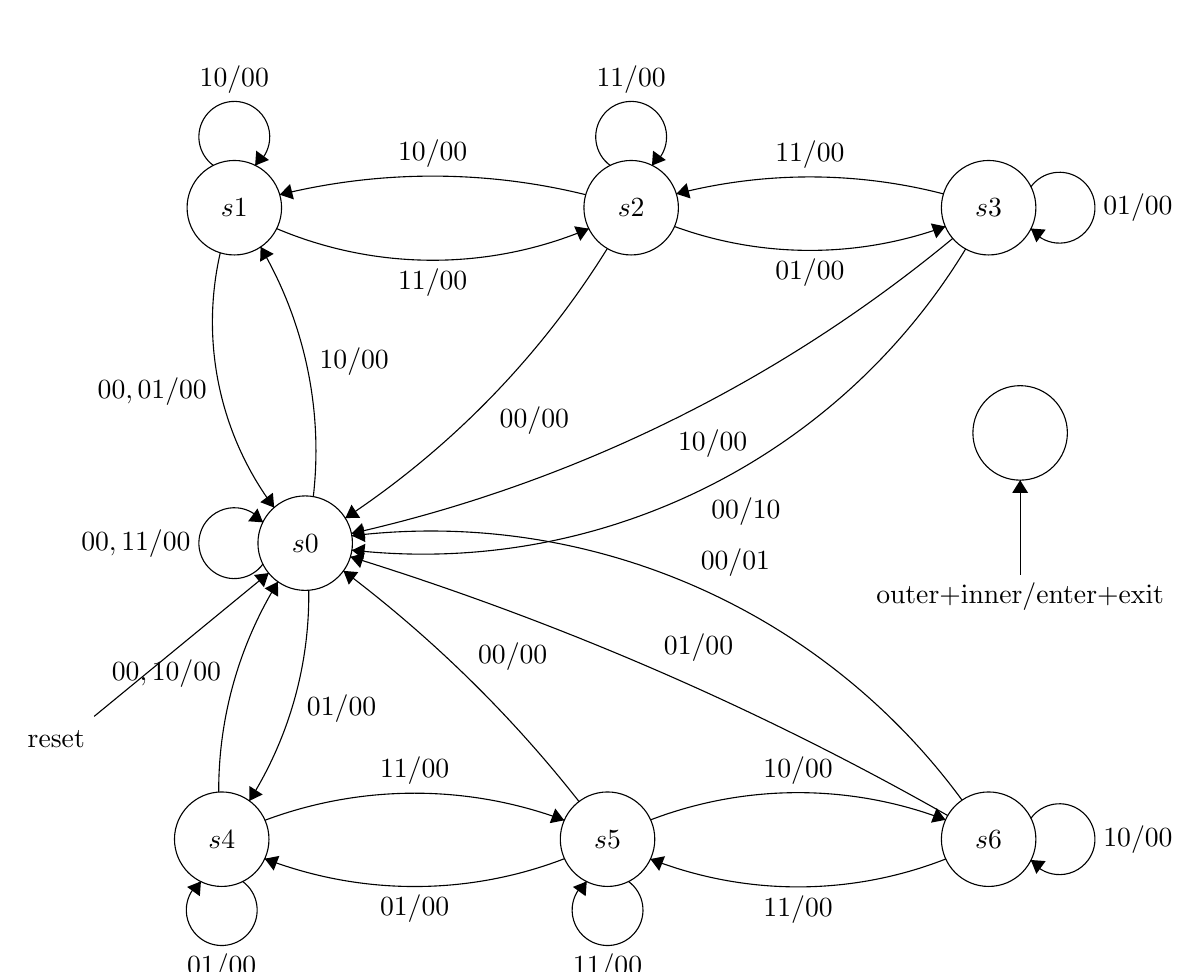
\begin{tikzpicture}[scale=0.2]
                \tikzstyle{every node}+=[inner sep=0pt]
                \draw [black] (24.3,-31.5) circle (3);
                \draw (24.3,-31.5) node {$s0$};
                \draw [black] (19.8,-10.2) circle (3);
                \draw (19.8,-10.2) node {$s1$};
                \draw [black] (45,-10.2) circle (3);
                \draw (45,-10.2) node {$s2$};
                \draw [black] (67.7,-10.2) circle (3);
                \draw (67.7,-10.2) node {$s3$};
                \draw [black] (19,-50.3) circle (3);
                \draw (19,-50.3) node {$s4$};
                \draw [black] (43.5,-50.3) circle (3);
                \draw (43.5,-50.3) node {$s5$};
                \draw [black] (67.7,-50.3) circle (3);
                \draw (67.7,-50.3) node {$s6$};
                \draw [black] (69.7,-24.5) circle (3);
                \draw [black] (21.467,-12.692) arc (30.42374:-6.5651:25.542);
                \fill [black] (21.47,-12.69) -- (21.44,-13.63) -- (22.3,-13.13);
                \draw (25.18,-20) node [right] {$10/00$};
                \draw [black] (21.62,-32.823) arc (-36:-324:2.25);
                \draw (17.05,-31.5) node [left] {$00,11/00$};
                \fill [black] (21.62,-30.18) -- (21.27,-29.3) -- (20.68,-30.11);
                \draw [black] (10.9,-42.5) -- (21.98,-33.4);
                \draw (10.34,-43.93) node [left] {reset};
                \fill [black] (21.98,-33.4) -- (21.05,-33.52) -- (21.68,-34.3);
                \draw [black] (42.312,-11.528) arc (-67.0876:-112.9124:25.459);
                \fill [black] (42.31,-11.53) -- (41.38,-11.38) -- (41.77,-12.3);
                \draw (32.4,-14.04) node [below] {$11/00$};
                \draw [black] (18.477,-7.52) arc (234:-54:2.25);
                \draw (19.8,-2.95) node [above] {$10/00$};
                \fill [black] (21.12,-7.52) -- (22,-7.17) -- (21.19,-6.58);
                \draw [black] (43.677,-7.52) arc (234:-54:2.25);
                \draw (45,-2.95) node [above] {$11/00$};
                \fill [black] (46.32,-7.52) -- (47.2,-7.17) -- (46.39,-6.58);
                \draw [black] (64.949,-11.393) arc (-69.9827:-110.0173:25.121);
                \fill [black] (64.95,-11.39) -- (64.03,-11.2) -- (64.37,-12.14);
                \draw (56.35,-13.41) node [below] {$01/00$};
                \draw [black] (66.239,-12.819) arc (-31.2914:-96.42652:40.325);
                \fill [black] (27.27,-31.95) -- (28,-32.53) -- (28.12,-31.54);
                \draw (52.29,-28.59) node [below] {$00/10$};
                \draw [black] (70.38,-8.877) arc (144:-144:2.25);
                \draw (74.95,-10.2) node [right] {$01/00$};
                \fill [black] (70.38,-11.52) -- (70.73,-12.4) -- (71.32,-11.59);
                \draw [black] (24.525,-34.49) arc (0.78771:-32.27558:24.425);
                \fill [black] (20.75,-47.87) -- (21.6,-47.46) -- (20.76,-46.92);
                \draw (24.38,-42) node [right] {$01/00$};
                \draw [black] (21.746,-49.096) arc (110.50165:69.49835:27.135);
                \fill [black] (40.75,-49.1) -- (40.18,-48.35) -- (39.83,-49.28);
                \draw (31.25,-46.88) node [above] {$11/00$};
                \draw [black] (20.323,-52.98) arc (54:-234:2.25);
                \draw (19,-57.55) node [below] {$01/00$};
                \fill [black] (17.68,-52.98) -- (16.8,-53.33) -- (17.61,-53.92);
                \draw [black] (18.809,-47.308) arc (-179.75617:-211.7317:25.191);
                \fill [black] (22.57,-33.95) -- (21.73,-34.37) -- (22.58,-34.9);
                \draw (18.99,-39.81) node [left] {$00,10/00$};
                \draw [black] (22.327,-29.244) arc (-143.20604:-192.93531:19.668);
                \fill [black] (22.33,-29.24) -- (22.25,-28.3) -- (21.45,-28.9);
                \draw (18.09,-21.88) node [left] {$00,01/00$};
                \draw [black] (46.235,-49.071) arc (110.91381:69.08619:26.235);
                \fill [black] (64.96,-49.07) -- (64.4,-48.32) -- (64.04,-49.25);
                \draw (55.6,-46.84) node [above] {$10/00$};
                \draw [black] (44.823,-52.98) arc (54:-234:2.25);
                \draw (43.5,-57.55) node [below] {$11/00$};
                \fill [black] (42.18,-52.98) -- (41.3,-53.33) -- (42.11,-53.92);
                \draw [black] (40.768,-51.535) arc (-68.92326:-111.07674:26.466);
                \fill [black] (21.73,-51.54) -- (22.3,-52.29) -- (22.66,-51.36);
                \draw (31.25,-53.81) node [below] {$01/00$};
                \draw [black] (64.977,-51.556) arc (-68.58801:-111.41199:25.686);
                \fill [black] (46.22,-51.56) -- (46.78,-52.31) -- (47.15,-51.38);
                \draw (55.6,-53.83) node [below] {$11/00$};
                \draw [black] (70.38,-48.977) arc (144:-144:2.25);
                \draw (74.95,-50.3) node [right] {$10/00$};
                \fill [black] (70.38,-51.62) -- (70.73,-52.5) -- (71.32,-51.69);
                \draw [black] (27.263,-31.033) arc (96.90441:36.25303:41.82);
                \fill [black] (27.26,-31.03) -- (28.12,-31.43) -- (28,-30.44);
                \draw (51.62,-33.64) node [above] {$00/01$};
                \draw [black] (22.683,-9.374) arc (103.8629:76.1371:40.554);
                \fill [black] (22.68,-9.37) -- (23.58,-9.67) -- (23.34,-8.7);
                \draw (32.4,-7.69) node [above] {$10/00$};
                \draw [black] (47.868,-9.322) arc (104.48223:75.51777:33.918);
                \fill [black] (47.87,-9.32) -- (48.77,-9.61) -- (48.52,-8.64);
                \draw (56.35,-7.74) node [above] {$11/00$};
                \draw [black] (26.73,-33.259) arc (53.03753:38.16866:80.908);
                \fill [black] (26.73,-33.26) -- (27.07,-34.14) -- (27.67,-33.34);
                \draw (37.48,-39.62) node [above] {$00/00$};
                \draw [black] (43.487,-12.79) arc (-31.83323:-56.52986:55.827);
                \fill [black] (26.85,-29.91) -- (27.79,-29.89) -- (27.24,-29.06);
                \draw (36.62,-23.72) node [right] {$00/00$};
                \draw [black] (27.172,-32.367) arc (72.75818:60.39926:192.01);
                \fill [black] (27.17,-32.37) -- (27.79,-33.08) -- (28.08,-32.13);
                \draw (49.28,-39.03) node [above] {$01/00$};
                \draw [black] (65.421,-12.15) arc (-50.39212:-77.32581:91.321);
                \fill [black] (27.24,-30.89) -- (28.13,-31.2) -- (27.91,-30.23);
                \draw (50.18,-24.29) node [below] {$10/00$};
                \draw [black] (69.7,-33.5) -- (69.7,-27.5);
                \draw (69.7,-34) node [below] {outer+inner/enter+exit};
                \fill [black] (69.7,-27.5) -- (69.2,-28.3) -- (70.2,-28.3);
                \end{tikzpicture}
                
                \caption{Car Detection FSM diagram}
            \end{figure} 
            Our state machine has 7 states. 
            \begin{description}
                \item[S0:] Both sensors are not triggered.
                \item[S1:] A car is starting to enter the lot.
                \item[S2:] A car is enterting the lot and triggering both sensors.
                \item[S3:] A car is entering the lot and is only triggering the inside sensor. 
                \item[S4:] A car is starting to exit the lot.
                \item[S5:] A car is exiting the lot and triggering both sensors.
                \item[S6:] A car is exiting the lot and only triggering the outside sensor.
            \end{description}
            Our FSM also accounts for pedestrians triggering the sensors. For example, if a car starts to enter the parking lot and triggers the outside sensor. A pedestrian could then trigger the inside sensor, but we don't want the pedestrian to mess up our detector so if the inside sensor then becomes untriggered then we know the car is still only triggering the outside sensor.

            \begin{figure}[!htb]
                \centering
                \captionsetup{justification=centering}
                
                \includegraphics[scale = 0.45]{Images/detectorFSM testbench.png}
                
                \caption{Car Detection Waveform}
            \end{figure}
            This testbench test every transition in the Car Detection FSM. We can see from the waveform that the enter signal is only high when the sensors go through the sequence $00 \rightarrow 10 \rightarrow 11 \rightarrow 01 \rightarrow 00$. We can also see the exit signal is only high when the sensors go through the sequence $00 \rightarrow 01 \rightarrow 11 \rightarrow 10 \rightarrow 00$.
        
        \subsection{Car Counter}
            The module to track the number of cars present in the garage receives inputs from the car detection module. It is flagged when a car has entered or exited the lot and then the current state of the counter is increased or decreased. The lot has a maximum of 16 spots so the counter stops tracking any signals after this. This applies to 0 as well as there cannot be negative cars in the lot. The output value is assigned the same value as the state.

            \begin{figure}[!htb]
                \centering
                \captionsetup{justification=centering}
                
                \includegraphics[scale=0.43]{Images/car counter testbench.png}
                
                \caption{Car Counter Waveform}
            \end{figure} 

            This testbench bench demonstrates the expected behavior of the car counter module. The count increments whever incr is high and decrements whenever decr is high. It also tests that the count stays the same when both signals are high or low. It also tests the bounds of the counter, 0 and 16.
        
        \subsection{Seven Segment Display}
            A module is dedicated to output the current count to the HEX display, it receives the count from the car counter module. Based on the count, it categorizes which state the system should be in, zero through sixteen, with a certain output designated for each state. When there are 16 cars in the lot, it outputs “FULL”, with zero cars in the lot it outputs “CLEAR0”, otherwise it displays the current number. This module is only combinational logic so there is no diagrams to provide.
        
        \subsection{DE1\_SoC}
            This is the top-level module in the system. It begins with initializing all the inputs and outputs that will be used in the parking lot occupancy counter. Then it assigns inputs for the sensors and reset and assigns outputs for the LEDs. Next, the system creates nets that will allow information and signals to be transmitted from the different devices in the system.

            \begin{figure}[!htb]
                \centering
                \captionsetup{justification=centering}
                
                \includegraphics[scale=0.6]{Images/Lab1 Block Diagram.pdf}
                
                \caption{Top-level Module Block Diagram}
            \end{figure} 
            \begin{figure}[!htb]
                \centering
                \captionsetup{justification=centering}
                
                \includegraphics[scale=0.4]{Images/top level module testbench.png}
                
                \caption{Top-level Module Waveform}
            \end{figure} 
            \newpage
            This waveform demonstrates the top level module has all the correct connections. When the switches are changed through the GPIO ports, the associated LEDs turn on. When the detector sees cars entering and exiting the counter changes accordingly. And when the count changes, so do the hex displays. 
            
    
    \section{Results}

        \subsection{Flow Summary}
            \begin{figure}[!htb]
                \centering
                \captionsetup{justification=centering}
                
                \includegraphics[scale=0.69]{Images/resource utilization.png}
                
                \caption{Resource Utilization}
            \end{figure} 
            
    \section{Experience Report}
        We found this lab to overall not be too challenging, but a great precursor to get us familiar with SystemVerilog after a break from using it. It was almost all encompassing with general functions and syntax that we will need to use for the rest of the quarter. The most difficult part for us was to ensure that the finite state machine in the car detection module could identify the differences between a car and person, then testing all the edge cases and inputs for the machine. Besides the tedious time spent figuring that out, there were not many other issues encountered.\\
        Although intuitive, we found it very useful to test each of the modules before moving on to implementing the next one. This allowed for us to pinpoint the module, and almost block of code, where an error occurs because the other modules have been tested and work as expected. \\
        This lab took us approximately 12 hours, broken down as follows:
        \begin{description}
            \item[Reading:] 30 minutes
            \item[Planning:] 30 minutes
            \item[Coding:] 5 hours
            \item[Testing:] 3 hours
            \item[Write up] 3 hours
        \end{description}        
    \end{document}
